\documentclass[tikz]{standalone}
\usetikzlibrary{positioning,shapes}

\begin{document}

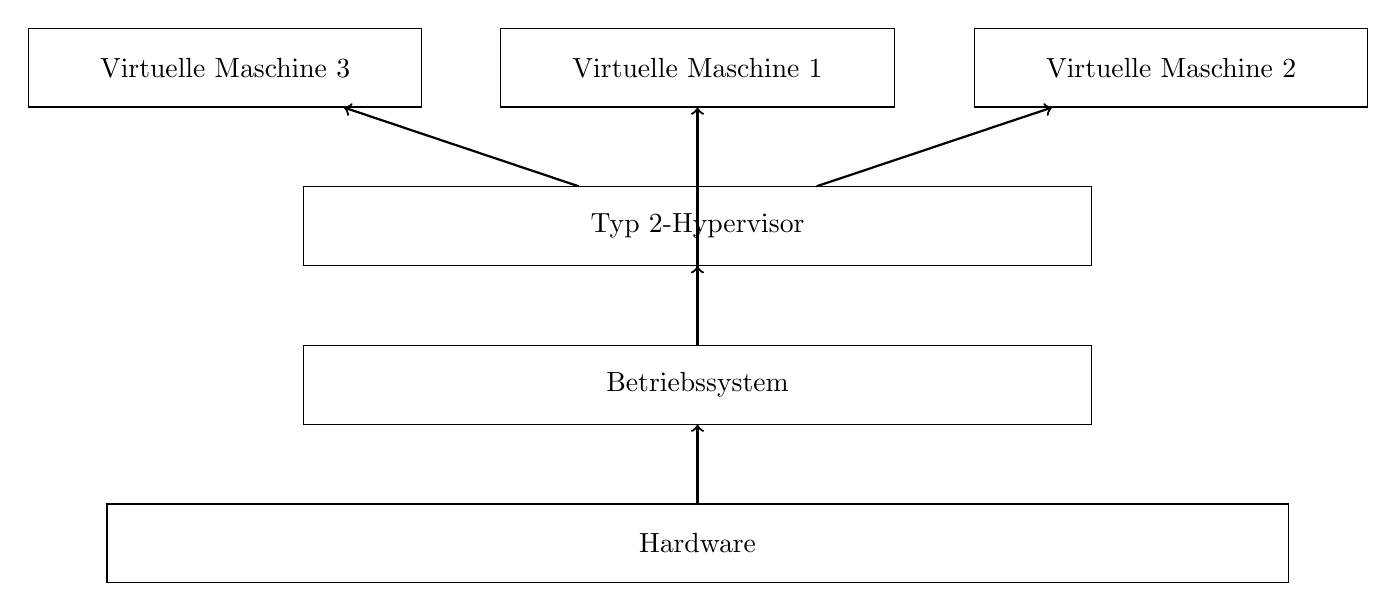
\begin{tikzpicture}[
    block1/.style={draw, fill=white, rectangle, minimum width=5cm, minimum height=1cm},
    block2/.style={draw, fill=white, rectangle, minimum width=15cm, minimum height=1cm},
    block3/.style={draw, fill=white, rectangle, minimum width=10cm, minimum height=1cm},
    arrow/.style={->, thick}
]
    % Blocks
    \node[block2] (hardware) {Hardware};
    \node[block3, above=of hardware] (OS) {Betriebssystem};
    \node[block3,left=1cm of OS ,above=of OS] (hypervisor) {Typ 2-Hypervisor};
   
    \node[block1, above=of hypervisor] (vm1) {Virtuelle Maschine 1};
    \node[block1, right=1cm of vm1] (vm2) {Virtuelle Maschine 2};
    \node[block1, left=7cm of vm2] (vm3) {Virtuelle Maschine 3};

    % Arrows
    \draw[arrow] (hardware) -- (OS);
    \draw[arrow] (OS) -- (vm1);
    \draw[arrow] (OS) -- (hypervisor);
    \draw[arrow] (hypervisor) -- (vm2);
    \draw[arrow] (hypervisor) -- (vm3);
\end{tikzpicture}

\end{document}